%Version 3.1 December 2024
% See section 11 of the User Manual for version history
%
%%%%%%%%%%%%%%%%%%%%%%%%%%%%%%%%%%%%%%%%%%%%%%%%%%%%%%%%%%%%%%%%%%%%%%
%%                                                                 %%
%% Please do not use \input{...} to include other tex files.       %%
%% Submit your LaTeX manuscript as one .tex document.              %%
%%                                                                 %%
%% All additional figures and files should be attached             %%
%% separately and not embedded in the \TeX\ document itself.       %%
%%                                                                 %%
%%%%%%%%%%%%%%%%%%%%%%%%%%%%%%%%%%%%%%%%%%%%%%%%%%%%%%%%%%%%%%%%%%%%%

%%\documentclass[referee,sn-basic]{sn-jnl}% referee option is meant for double line spacing

%%=======================================================%%
%% to print line numbers in the margin use lineno option %%
%%=======================================================%%

%%\documentclass[lineno,pdflatex,sn-basic]{sn-jnl}% Basic Springer Nature Reference Style/Chemistry Reference Style

%%=========================================================================================%%
%% the documentclass is set to pdflatex as default. You can delete it if not appropriate.  %%
%%=========================================================================================%%

%%\documentclass[sn-basic]{sn-jnl}% Basic Springer Nature Reference Style/Chemistry Reference Style

%%Note: the following reference styles support Namedate and Numbered referencing. By default the style follows the most common style. To switch between the options you can add or remove “Numbered” in the optional parenthesis. 
%%The option is available for: sn-basic.bst, sn-chicago.bst%  
 
%%\documentclass[pdflatex,sn-nature]{sn-jnl}% Style for submissions to Nature Portfolio journals
%%\documentclass[pdflatex,sn-basic]{sn-jnl}% Basic Springer Nature Reference Style/Chemistry Reference Style
\documentclass[pdflatex,sn-mathphys-num]{sn-jnl}% Math and Physical Sciences Numbered Reference Style
%%\documentclass[pdflatex,sn-mathphys-ay]{sn-jnl}% Math and Physical Sciences Author Year Reference Style
%%\documentclass[pdflatex,sn-aps]{sn-jnl}% American Physical Society (APS) Reference Style
%%\documentclass[pdflatex,sn-vancouver-num]{sn-jnl}% Vancouver Numbered Reference Style
%%\documentclass[pdflatex,sn-vancouver-ay]{sn-jnl}% Vancouver Author Year Reference Style
%%\documentclass[pdflatex,sn-apa]{sn-jnl}% APA Reference Style
%%\documentclass[pdflatex,sn-chicago]{sn-jnl}% Chicago-based Humanities Reference Style

%%%% Standard Packages
%%<additional latex packages if required can be included here>

\usepackage{graphicx}%
\usepackage{multirow}%
\usepackage{amsmath,amssymb,amsfonts}%
\usepackage{amsthm}%
\usepackage{mathrsfs}%
\usepackage[title]{appendix}%
\usepackage{xcolor}%
\usepackage{textcomp}%
\usepackage{manyfoot}%
\usepackage{booktabs}%
\usepackage{algorithm}%
\usepackage{algorithmicx}%
\usepackage{algpseudocode}%
\usepackage{listings}%
\usepackage[utf8]{inputenc}
\usepackage{bm}
\usepackage{caption}
\usepackage{needspace}

%%%%

%%%%%=============================================================================%%%%
%%%%  Remarks: This template is provided to aid authors with the preparation
%%%%  of original research articles intended for submission to journals published 
%%%%  by Springer Nature. The guidance has been prepared in partnership with 
%%%%  production teams to conform to Springer Nature technical requirements. 
%%%%  Editorial and presentation requirements differ among journal portfolios and 
%%%%  research disciplines. You may find sections in this template are irrelevant 
%%%%  to your work and are empowered to omit any such section if allowed by the 
%%%%  journal you intend to submit to. The submission guidelines and policies 
%%%%  of the journal take precedence. A detailed User Manual is available in the 
%%%%  template package for technical guidance.
%%%%%=============================================================================%%%%

%% as per the requirement new theorem styles can be included as shown below
\theoremstyle{thmstyleone}%
\newtheorem{theorem}{Theorem}%  meant for continuous numbers
%%\newtheorem{theorem}{Theorem}[section]% meant for sectionwise numbers
%% optional argument [theorem] produces theorem numbering sequence instead of independent numbers for Proposition
\newtheorem{proposition}[theorem]{Proposition}% 
%%\newtheorem{proposition}{Proposition}% to get separate numbers for theorem and proposition etc.

\theoremstyle{thmstyletwo}%
\newtheorem{example}{Example}%
\newtheorem{remark}{Remark}%

\theoremstyle{thmstylethree}%
\newtheorem{definition}{Definition}%

\raggedbottom
%%\unnumbered% uncomment this for unnumbered level heads

\lstset{
    basicstyle=\ttfamily\footnotesize,
    keywordstyle=\color{black},
    commentstyle=\color{black},
    stringstyle=\color{black},
    identifierstyle=\color{black},
    numberstyle=\color{black},
    emphstyle=\color{black},
    numbers=none,
    frame=single,
    breaklines=true,
    columns=fullflexible,
    keepspaces=true,
    showstringspaces=false,
    captionpos=b
}

\captionsetup[lstlisting]{
    labelformat=empty,
    position=bottom
}

\begin{document}

\title[Automated Multi Component Prompt Optimization for Lightweight LLMs]{Automated Multi Component Prompt Optimization for Lightweight LLMs}

\author{\fnm{Marcello} \sur{Calza}}\email{marcello.calza@studenti.unimi.it}

%%\affil*[1]{\orgdiv{Department}, \orgname{University}, \orgaddress{\city{City}, \country{Italy}}}

\abstract{}

%%\keywords{}

\maketitle

\textit{Parts of this projects have been developed with the assistance of OpenAI’s ChatGPT (GPT-5). The AI was used to support the development of the code, the drafting and summarization of descriptive texts. All content produced with AI assistance has been carefully reviewed, edited, and validated by me. I take full responsibility for the final content and its accuracy, relevance, and academic integrity.}
\clearpage

\section{Introduction}

The project implements an automated prompt optimization pipeline for
lightweight Large Language Models (LLMs), with the objective of improving
their performance on different natural language processing tasks through
iterative prompt modification and evaluation.

The pipeline is designed to operate on quantized models with approximately
8 billion parameters, allowing prompt optimization experiments to be
conducted using locally executed language models. The optimization process
is evaluated across multiple models and tasks, making it possible to
compare the effects of prompt optimization under different model
architectures and task complexities.

The experimental evaluation focuses on two tasks: logical deduction and
sentiment classification. These tasks were selected to represent different
levels of difficulty, allowing the effectiveness of prompt optimization to
be investigated on both a relatively simple classification problem and a
more complex reasoning problem.

\section{Research question and methodology}\label{sec:method}

\subsection{Prompt Representation and Initialization (\texttt{init\_prompts.py})}

Three initial prompting strategies are manually designed for each of the
two tasks: zero-shot, chain-of-thought (CoT), and few-shot prompting.
Each prompt is represented through three components: \textit{instruction},
\textit{reasoning}, and \textit{examples}. The instruction is the basic
natural-language command that directly tells the model what task to perform.
Task-specific output constraints are appended separately when the complete
model input is assembled.

\begin{itemize}
    \item \textbf{Zero-shot:} Contains only the task-specific instruction.

    \item \textbf{CoT:} Adds task-specific reasoning steps to the instruction.

    \item \textbf{Few-shot:} Adds task-specific labeled examples to the
    instruction.
\end{itemize}

For logical deduction, the CoT prompt guides the model through constraint
extraction, relationship construction, consistency checking, and answer
identification. For sentiment classification, it guides the model through
the identification and interpretation of sentiment-related expressions.

The few-shot templates contain task-specific examples designed to
illustrate the corresponding task: two examples are included for logical
deduction and three examples for sentiment classification.

A prompt is represented as a structured \texttt{PromptObject} holding these
components. It is rendered by combining the available components or returned
directly when it is a raw prompt. In both cases, the output constraints are
appended to the rendered prompt to specify the required response format.

\subsection{Prompt Optimization Methodology(\texttt{MultiBranchOptimizer.py})}

Prompt optimization is performed by the \texttt{MultiBranchOptimizer}
class. The search is launched through its \texttt{optimize()} method, which
initializes the candidate pool and then runs the iterative search. The optimizer
generates prompt variants, evaluates their performance on the optimization
dataset, and retains the best-performing candidates in a top-\(k\) pool.

Formally, let \(M\) be a language model, and let \(\mathcal{D}_{\text{opt}}\) and 
\(\mathcal{D}_{\text{test}}\) be the optimization and held-out sets of a task. 
A prompt is a triple \(p=(\iota,\rho,\varepsilon)\) of instruction, reasoning steps, 
and examples (or a raw text, in the case of the rewrite branch), and its score 
\(s(p;\mathcal{D})\) is the mean keyword-matching score obtained by \(M\) on a dataset 
\(\mathcal{D}\) when prompted with \(p\). Given an initial prompt \(p_0\), the goal is 
to find
\begin{equation}
p^{\ast}=\arg\max_{p\in\mathcal{P}(p_0)} s(p;\mathcal{D}_{\text{opt}}),
\end{equation}
where \(\mathcal{P}(p_0)\) is the set of prompts reachable from \(p_0\) through the 
mutation operators. The quality of \(p^{\ast}\) is then assessed by comparing 
\(s(p^{\ast};\mathcal{D}_{\text{test}})\) with \(s(p_0;\mathcal{D}_{\text{test}})\).

The optimization process combines multiple prompt mutation strategies
with failure analysis, which is used to identify weaknesses in the
current prompt and guide subsequent modifications.

\subsubsection{Multi-Branch Optimization}

The optimizer supports different strategies for modifying prompts.
Each strategy targets either the complete prompt or a specific
component of a structured \texttt{PromptObject}. The organization of the
prompt into components was inspired by the division of the prompt in multiple 
optimizable sentences by Hsieh et al.~\cite{hsieh2024}, although
the division in components is much simpler.

\begin{itemize}

    \item \textbf{Rewrite:} Rewrites the entire prompt as a single raw
          text, without preserving the structured components of a
          \texttt{PromptObject}. This approach corresponds to a
          free-form optimization strategy in which the mutation model
          is asked to improve the complete prompt.

    \item \textbf{Instruction:} Rewrites only the instruction field of
          a structured prompt, without modifying its reasoning
          steps or examples.

    \item \textbf{CoT:} Adds reasoning steps to the reasoning field if
          it is empty, or improves the existing steps if they are
          already present.

    \item \textbf{Examples:} Adds two new examples to the examples
          field, up to a maximum of 10 shots, inspired by the prompts
          with large numbers of shots reported by Schulhoff et
          al.~\cite{schulhoff2024}, or improves the existing examples when the maximum
          number of shots has been reached.

\end{itemize}

The instruction, CoT, and examples branches can be activated
simultaneously within the same optimizer instance. When all
three branches are active, each selected parent prompt generates
three separate candidates, one for each branch. Each candidate
modifies only its corresponding component of the parent prompt,
while preserving the remaining components. All generated
candidates are evaluated independently.

The rewrite branch instead operates on the complete prompt and is
independent of the structured component-based optimization. Candidate
generation is handled by \texttt{mutate()}, which collects failed cases for
the selected parent, obtains a failure analysis, and uses it to generate
child prompts for the active branches. These children are then evaluated,
and the candidate pool is updated by \texttt{optimize()}.

%%\vspace{1em}

%%\Needspace{20\baselineskip}
%%\begin{lstlisting}[
      %%caption={Instruction branch mutation prompt used to improve
      %%the instruction component based on the failure analysis.},
      %%label={lst:instruction-mutation},
  %%]
  %%You are optimizing ONLY the current prompt INSTRUCTION field.
  
  %%# CURRENT PROMPT:
  %%{full_prompt_context}
  
 %% # FAILURE ANALYSIS (NOT PART OF THE PROMPT):
  %%{failure_analysis}
  
  %%# TASK EXPLANATION (NOT PART OF THE PROMPT):
  %%{reference_block}
  
  %%#
  %%Do NOT rewrite or return REASONING.
  %%Do NOT rewrite or return EXAMPLES.
  %%Do NOT rewrite or return OUTPUT CONSTRAINTS.
  
  %%IMPROVE ONLY the INSTRUCTION with the goal of addressing the failure
  %%patterns identified by the FAILURE ANALYSIS.
  %%Preserve effective parts of the existing INSTRUCTION.
  %%Prioritize improving performance on unseen instances over making the prompt
  %%substantially different.
  %%The INSTRUCTION must NOT describe a step-by-step solving procedure.
  %%The INSTRUCTION may specify goals, priorities, constraints, or cautions.
  %%The INSTRUCTION must be applicable to ALL task instances.
  
  %%Return ONLY the rewritten INSTRUCTION.
  %%DO NOT include other text.
  %%DO NOT explain your reasoning.
%%\end{lstlisting}

%%\vspace{1em}

\subsubsection{Failure Analysis}

Before generating mutations, the optimizer analyzes the errors
produced by the current parent prompt, following the idea of including
failure cases in the prompt used to guide the optimization~\cite{ye2024}. 
The \texttt{collect\_failures()} function extracts incorrectly solved examples 
from the evaluation results and selects up to a maximum of 10 failures.

The \texttt{analyze\_failures()} function then constructs a prompt
containing the current parent prompt and the selected failure cases,
including the model predictions and expected outputs. The mutation
model is asked to identify up to three generalizable failure patterns,
supported either by multiple examples or by a clearly diagnostic
failure case.

For each identified pattern, the analysis must describe the observed
error, provide supporting evidence from the failure cases, and
identify which aspects of the current prompt may be insufficient
to prevent the error.

The resulting failure analysis is provided to the mutation model
together with the current prompt when generating the next candidate.
The selected mutation strategy is therefore guided by the weaknesses
identified in the previous evaluation.

\subsubsection{Optimization Algorithm}

The optimization algorithm maintains a pool of the \(k\) best
performing prompts, where \(k=5\) in all experiments, in a manner
inspired by the beam search algorithm of Hsieh et al.~\cite{hsieh2024}. 
This top-\(k\) selection strategy provides a compromise between greedy
optimization, which retains and mutates only the current best candidate, 
and population-based approaches that mutate a larger set of candidates.

Algorithm~\ref{alg:optimizer} summarizes the procedure. The pool is 
initialized through the \texttt{initialize\_population()} function with a 
chain of mutations starting from the baseline prompt: 
at each step the active branches generate one candidate each, and the 
best-performing child becomes the parent of the next step. In each 
subsequent generation, the parent is drawn uniformly at random from the 
current pool. When the instruction, CoT, and examples branches are all 
active, \texttt{crossover()} is also applied: a new structured prompt 
is built by independently selecting the instruction, reasoning, and examples 
fields from either of two randomly selected parents from the top-\(k\) pool. 
Crossover is an additional operation of the optimizer rather than a
separate mutation branch.

 
\begin{algorithm}[htbp]
      \caption{Multi-branch top-\(k\) prompt optimization}\label{alg:optimizer}
      \begin{algorithmic}[1]
      \Require initial prompt \(p_0\), optimization set \(\mathcal{D}_{\text{opt}}\), active branches \(\mathcal{B}\), pool size \(k\), maximum generations \(G\), patience \(\tau\)
      \Ensure optimized prompt \(p^{\ast}\)
      \State \(\mathcal{C}\gets\{p_0\}\); \(p\gets p_0\) \Comment{pool initialization}
      \While{\(|\mathcal{C}|<k\) and new candidates can be generated}
        \State \(\mathcal{F}\gets\textsc{Analyze}(p,\mathcal{D}_{\text{opt}})\) \Comment{failure analysis of the parent}
        \State \(\mathcal{N}\gets\{\textsc{Mutate}_b(p,\mathcal{F}) : b\in\mathcal{B}\}\)
        \State \(\mathcal{C}\gets\mathcal{C}\cup\mathcal{N}\); \(p\gets\arg\max_{c\in\mathcal{N}} s(c;\mathcal{D}_{\text{opt}})\)
      \EndWhile
      \State \(\mathcal{P}\gets\) the \(k\) best prompts of \(\mathcal{C}\) after removing duplicates
      \For{\(g=1,\dots,G\)}
        \State sample \(p\sim\mathcal{U}(\mathcal{P})\)
        \State \(\mathcal{F}\gets\textsc{Analyze}(p,\mathcal{D}_{\text{opt}})\) \Comment{failure analysis of the parent}
        \State \(\mathcal{N}\gets\{\textsc{Mutate}_b(p,\mathcal{F}) : b\in\mathcal{B}\}\)
        \If{instruction, CoT, and examples branches are active and \(|\mathcal{P}|\ge 2\)}
          \State sample two parents \(p_a,p_b\) from \(\mathcal{P}\); \(\mathcal{N}\gets\mathcal{N}\cup\{\textsc{Crossover}(p_a,p_b)\}\)
        \EndIf
        \State \(\mathcal{P}\gets\) the \(k\) best prompts of \(\mathcal{P}\cup\mathcal{N}\) after removing duplicates
        \If{the best score in \(\mathcal{P}\) has not improved for \(\tau\) generations}
          \State \textbf{break} \Comment{early stopping}
        \EndIf
      \EndFor
      \State \Return the best prompt in \(\mathcal{P}\)
      \end{algorithmic}
\end{algorithm}

\paragraph{Reproducibility.}

The optimizer uses a fixed base seed, consistent with the seed used for 
dataset partitioning and model evaluation, and distinct seeds are derived 
for successive mutation-model calls by adding a generation counter to the 
base seed (\texttt{get\_next\_seed()}). Results of candidate evaluations are 
cached to avoid redundant evaluations, and duplicate prompts are detected 
through a normalized hash (\texttt{normalize\_prompt()}).

\section{Experimental results}

\subsection{Models}

Three 8-billion-parameter language models are used in the experiments: 
\textbf{Qwen3-8B}~\cite{hf-qwen}, \textbf{Llama 3.1 8B Instruct}~\cite{hf-llama}, 
and \textbf{Ministral 8B Instruct}~\cite{hf-ministral}. All three models 
are used in the GGUF format with Q4\_K\_M quantization. This configuration 
reduces model storage and memory requirements while allowing the experiments 
to be performed locally.

\subsection{Benchmark Tasks}

Two benchmark tasks are selected for the optimization experiments.

\paragraph{Logical deduction: Five Objects.}

The first task is the \textit{Five Objects} logical deduction task from the
BIG-Bench benchmark. It presents a logical problem involving relationships
between objects, such as ordering, positions, rankings, or spatial
relationships, together with a set of five possible answers.

\paragraph{Sentiment classification: Sentiment140.}

The second task is the Sentiment140 tweet classification task from the
Natural Instructions dataset. Given a tweet, the model must classify its
sentiment as either positive or negative.

\paragraph{Task Selection Rationale.}

The two tasks were selected to investigate prompt optimization under 
different levels of task complexity: sentiment classification is a 
comparatively simple task in which short texts must be assigned to one 
of two categories, whereas the Five Objects task requires the model to 
reason about relationships and constraints. 
By applying the same optimization pipeline to both tasks, the experiments 
aim to examine whether prompt optimization produces different performance 
improvements depending on the complexity and nature of the task.

\subsection{Datasets and Data Preparation}\label{subsec:datasets}

The datasets introduced above are converted into standardized 
representations suitable for prompt construction and evaluation.
For each example, the context, answer choices, question, and correct 
answer (logical deduction) or the tweet text and sentiment label 
(sentiment classification) are extracted, and a task-specific output 
constraint is assigned, requiring the model to return only the expected 
answer without additional text.

Both datasets are then shuffled using a fixed random seed of 
\texttt{24052026} and divided into an optimization set and a held-out 
test set. For each task, the first 300 examples (75\%) are used during 
prompt optimization, while the following 100 examples (25\%) are reserved 
for evaluation on unseen data.

\subsection{Evaluation Methodology (\texttt{evaluator.py})}

The evaluation module measures model performance by comparing generated
predictions with the expected outputs. It is used both during the prompt
optimization process, to evaluate candidate prompts, and in the final
evaluation on the held-out test sets, to measure the effectiveness of
the optimizations on unseen examples.

Three evaluation metrics are implemented:

\begin{itemize}

    \item \textbf{Exact match:} Compares the normalized prediction with
          the expected output.

    \item \textbf{Keyword match:} Identifies the last valid answer label
          appearing in the prediction and checks whether it matches the
          expected output. This approach accounts for cases in which
          models do not strictly follow the output constraints and
          provide an explanation containing multiple answer labels.

    \item \textbf{LLM-based judging:} Uses a separate language model to
          assess whether the prediction matches the correct answer.

\end{itemize}

Although all three metrics are implemented, only keyword matching is
used in the experiments. The evaluation score is computed as the mean
of the individual example scores across the dataset.

\subsection{Experimental Results and Analysis}

The experiments investigate prompt optimization across two benchmark
tasks, three language models, three initial prompting strategies, and
five optimization configurations. The optimization stage uses the
300-example optimization subset introduced in Section~\ref{subsec:datasets}, 
while theeffectiveness of the final prompts is evaluated independently 
on the 100-example held-out test subset.

\subsubsection{Experimental Setup (\texttt{run\_optimization.py})}

For each language model, the same experimental configuration is
executed independently on both tasks. Each initial prompting strategy
is paired with every optimization configuration, resulting in the full
Cartesian product of initial prompts and optimizers.

For every model and task, this corresponds to
\(3\times5=15\) optimization runs. Across the three models, each task therefore
contains 45 optimization runs, for a total of 90 optimization runs
across the two tasks. The baseline prompts and the optimizers final generations prompts 
are additionally evaluated on the corresponding held-out test sets.

The optimizer configurations used in the experiments are the
following:

\begin{itemize}

\item \textbf{Rewrite}: full prompt rewriting using the
      \texttt{rewrite} branch.

\item \textbf{Instruction}: modification of only the instruction
      field.

\item \textbf{CoT}: modification of only the reasoning field.

\item \textbf{Examples}: modification of only the examples field.

\item \textbf{Multi}: simultaneous activation of the instruction,
      CoT, and examples branches.

\end{itemize}

The multi configuration does not activate the rewrite branch. It uses
the three structured branches and therefore also enables the crossover
operation described in Section~\ref{sec:method}.

All optimizers are configured with 300 optimization examples,
\(k=5\), a patience of 30 generations, and the common random seed
\texttt{24052026}. The experiment runner uses a maximum of 50
optimization generations through the default value of
\texttt{run\_experiments()}.

\subsubsection{Analysis Module and Visualization Procedure (\texttt{analysis.py})}

For each task and model, the generation-level results, the held-out 
test results, and the mutation records are stored as CSV files. 
The analysis produces three complementary views of the optimization 
process: generation-level score evolution, held-out test performance, 
and mutation-level improvement frequency.

\paragraph{Optimization-Set Performance}

The first result analysis concerns the 300-example optimization
dataset used during prompt search. The corresponding optimization-evolution
plots are stored in the \texttt{analysis/optimization\_evolution/} folder of the
repository. Across both tasks, the improvement
over the corresponding initial prompt was generally small. When an
optimization strategy succeeded in finding a better prompt, the
increase was typically in the order of a few hundredths, approximately
$0.01$ to $0.04$. In several configurations, no generated prompt
exceeded the initial optimization score throughout the optimization
process.

This behavior can also be observed in the optimization-evolution
plots. The curves generally show relatively small vertical changes
across generations, and in configurations where no improvement is
found, the best retained score remains at the initial level. The
plots also show that the different optimization branches do not
produce identical trajectories: some branches find improvements
earlier, while others remain nearly flat.

%%\begin{figure}[htbp]
%%\centering
%%\IfFileExists{../analysis/optimization_evolution/sentiment_cot_optimization_evolution.png}{
%%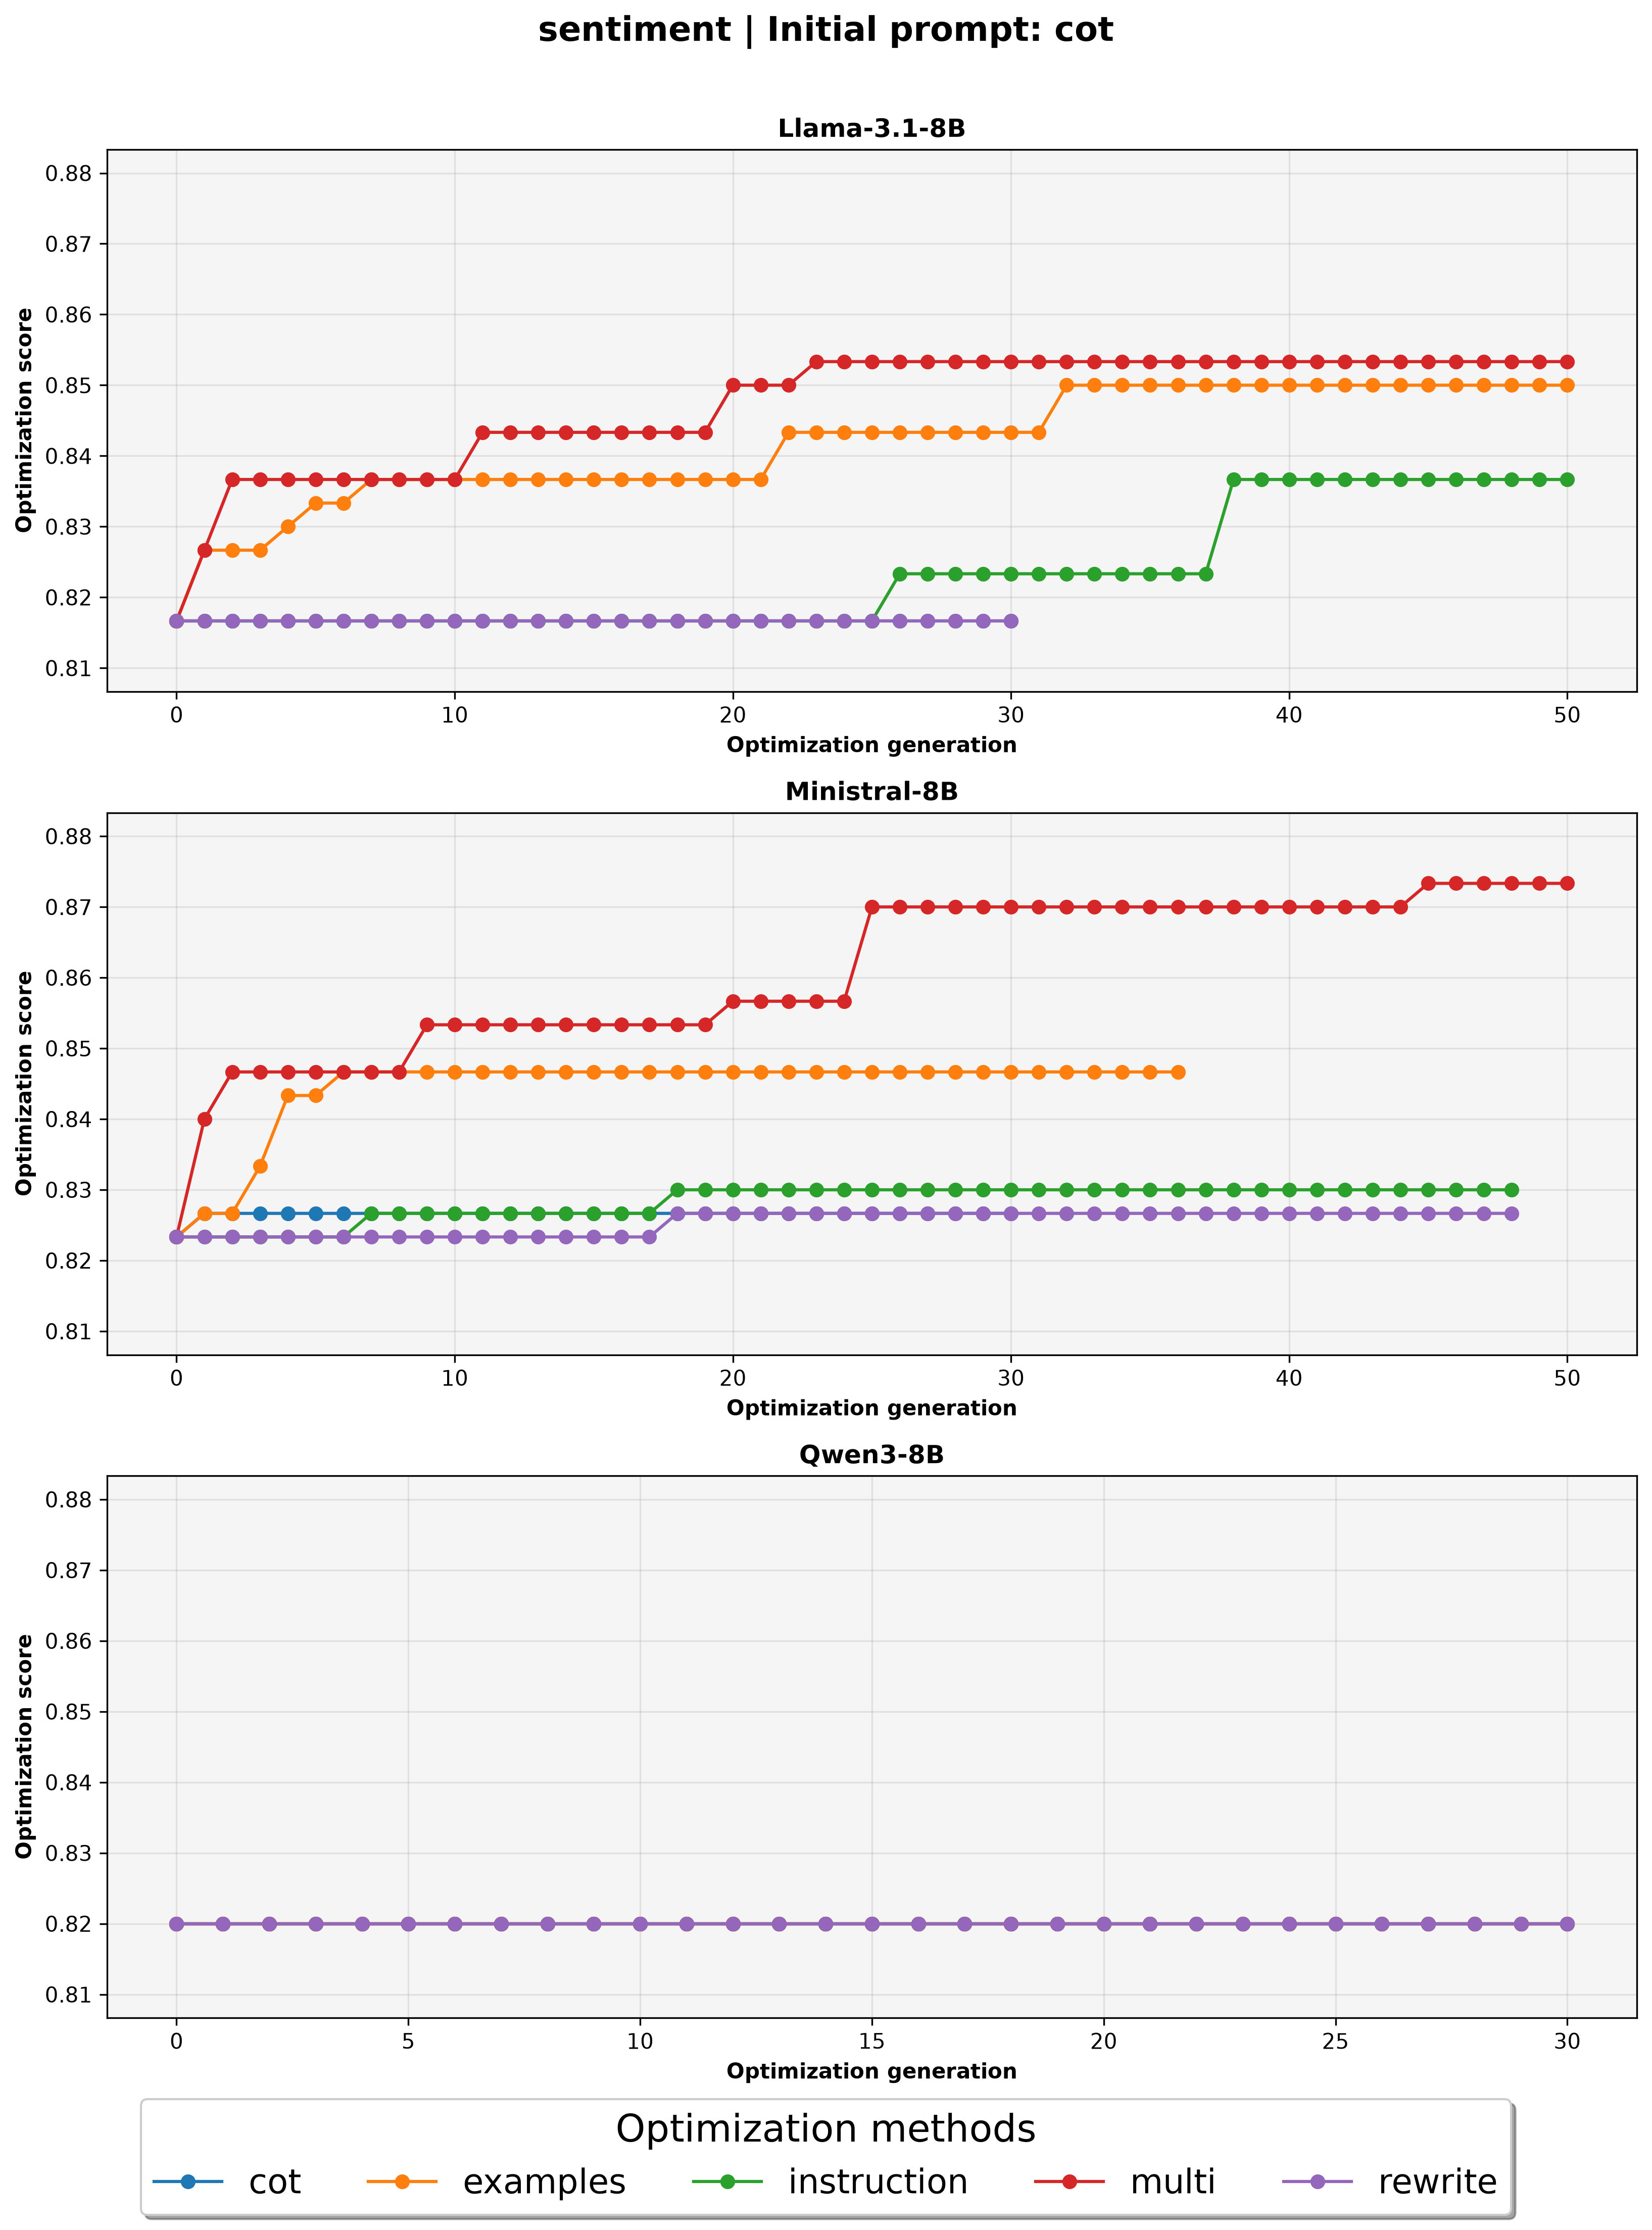
\includegraphics[width=\textwidth]{../analysis/optimization_evolution/sentiment_cot_optimization_evolution.png}
%%}{}
%%\caption{Evolution of optimization-set performance for the
%%sentiment task starting from the CoT prompt.}
%%\label{fig:optimization_evolution}
%%\end{figure}

For sentiment classification, the models were broadly comparable in terms
of their initial performance on the optimization set. The multi-branch 
configuration produced the largest improvement for Llama and Ministral 
from the CoT and zero-shot prompts and for all three models from the 
few-shot prompt, usually followed by the examples branch, while the 
full-prompt rewrite was particularly effective for Ministral from the 
few-shot prompt. For Qwen, none of the configurations exceeded the 
baseline from the CoT and zero-shot prompts.

The logical deduction task displayed greater variation between models. 
The multi-branch configuration was the strongest strategy for all three 
models from the CoT and zero-shot prompts, with the examples branch second 
from the zero-shot prompt. From the few-shot prompt, rewrite was strongest 
for Llama and Qwen, whereas the multi-branch configuration was strongest 
for Ministral, with the examples branch consistently among the stronger 
configurations.

These observations show that the multi-branch strategy was frequently 
effective at increasing optimization-set performance, particularly for 
zero-shot and CoT prompts. However, its effect was model and task dependent 
rather than universal.

\paragraph{Held-Out Test Performance}

The optimization-set results alone do not determine whether an
optimized prompt generalizes to unseen examples. For this reason, the
final prompt retained by each optimization run is evaluated
independently on the 100-example held-out test set. The corresponding
test-score plots are stored in the \texttt{analysis/test\_scores/} folder of the
repository.

Across the complete set of experiments, the held-out results show that
optimization-set improvements do not transfer uniformly to unseen data.
Some optimized prompts produce clear improvements over their initial
baselines, while others remain close to the baseline or perform worse.
The magnitude and direction of the change depend on the model, task,
initial prompting strategy, and optimization configuration.

%%\begin{figure}[htbp]
%%\centering
%%\IfFileExists{../analysis/test_scores/logical_cot_test_scores.png}{
%%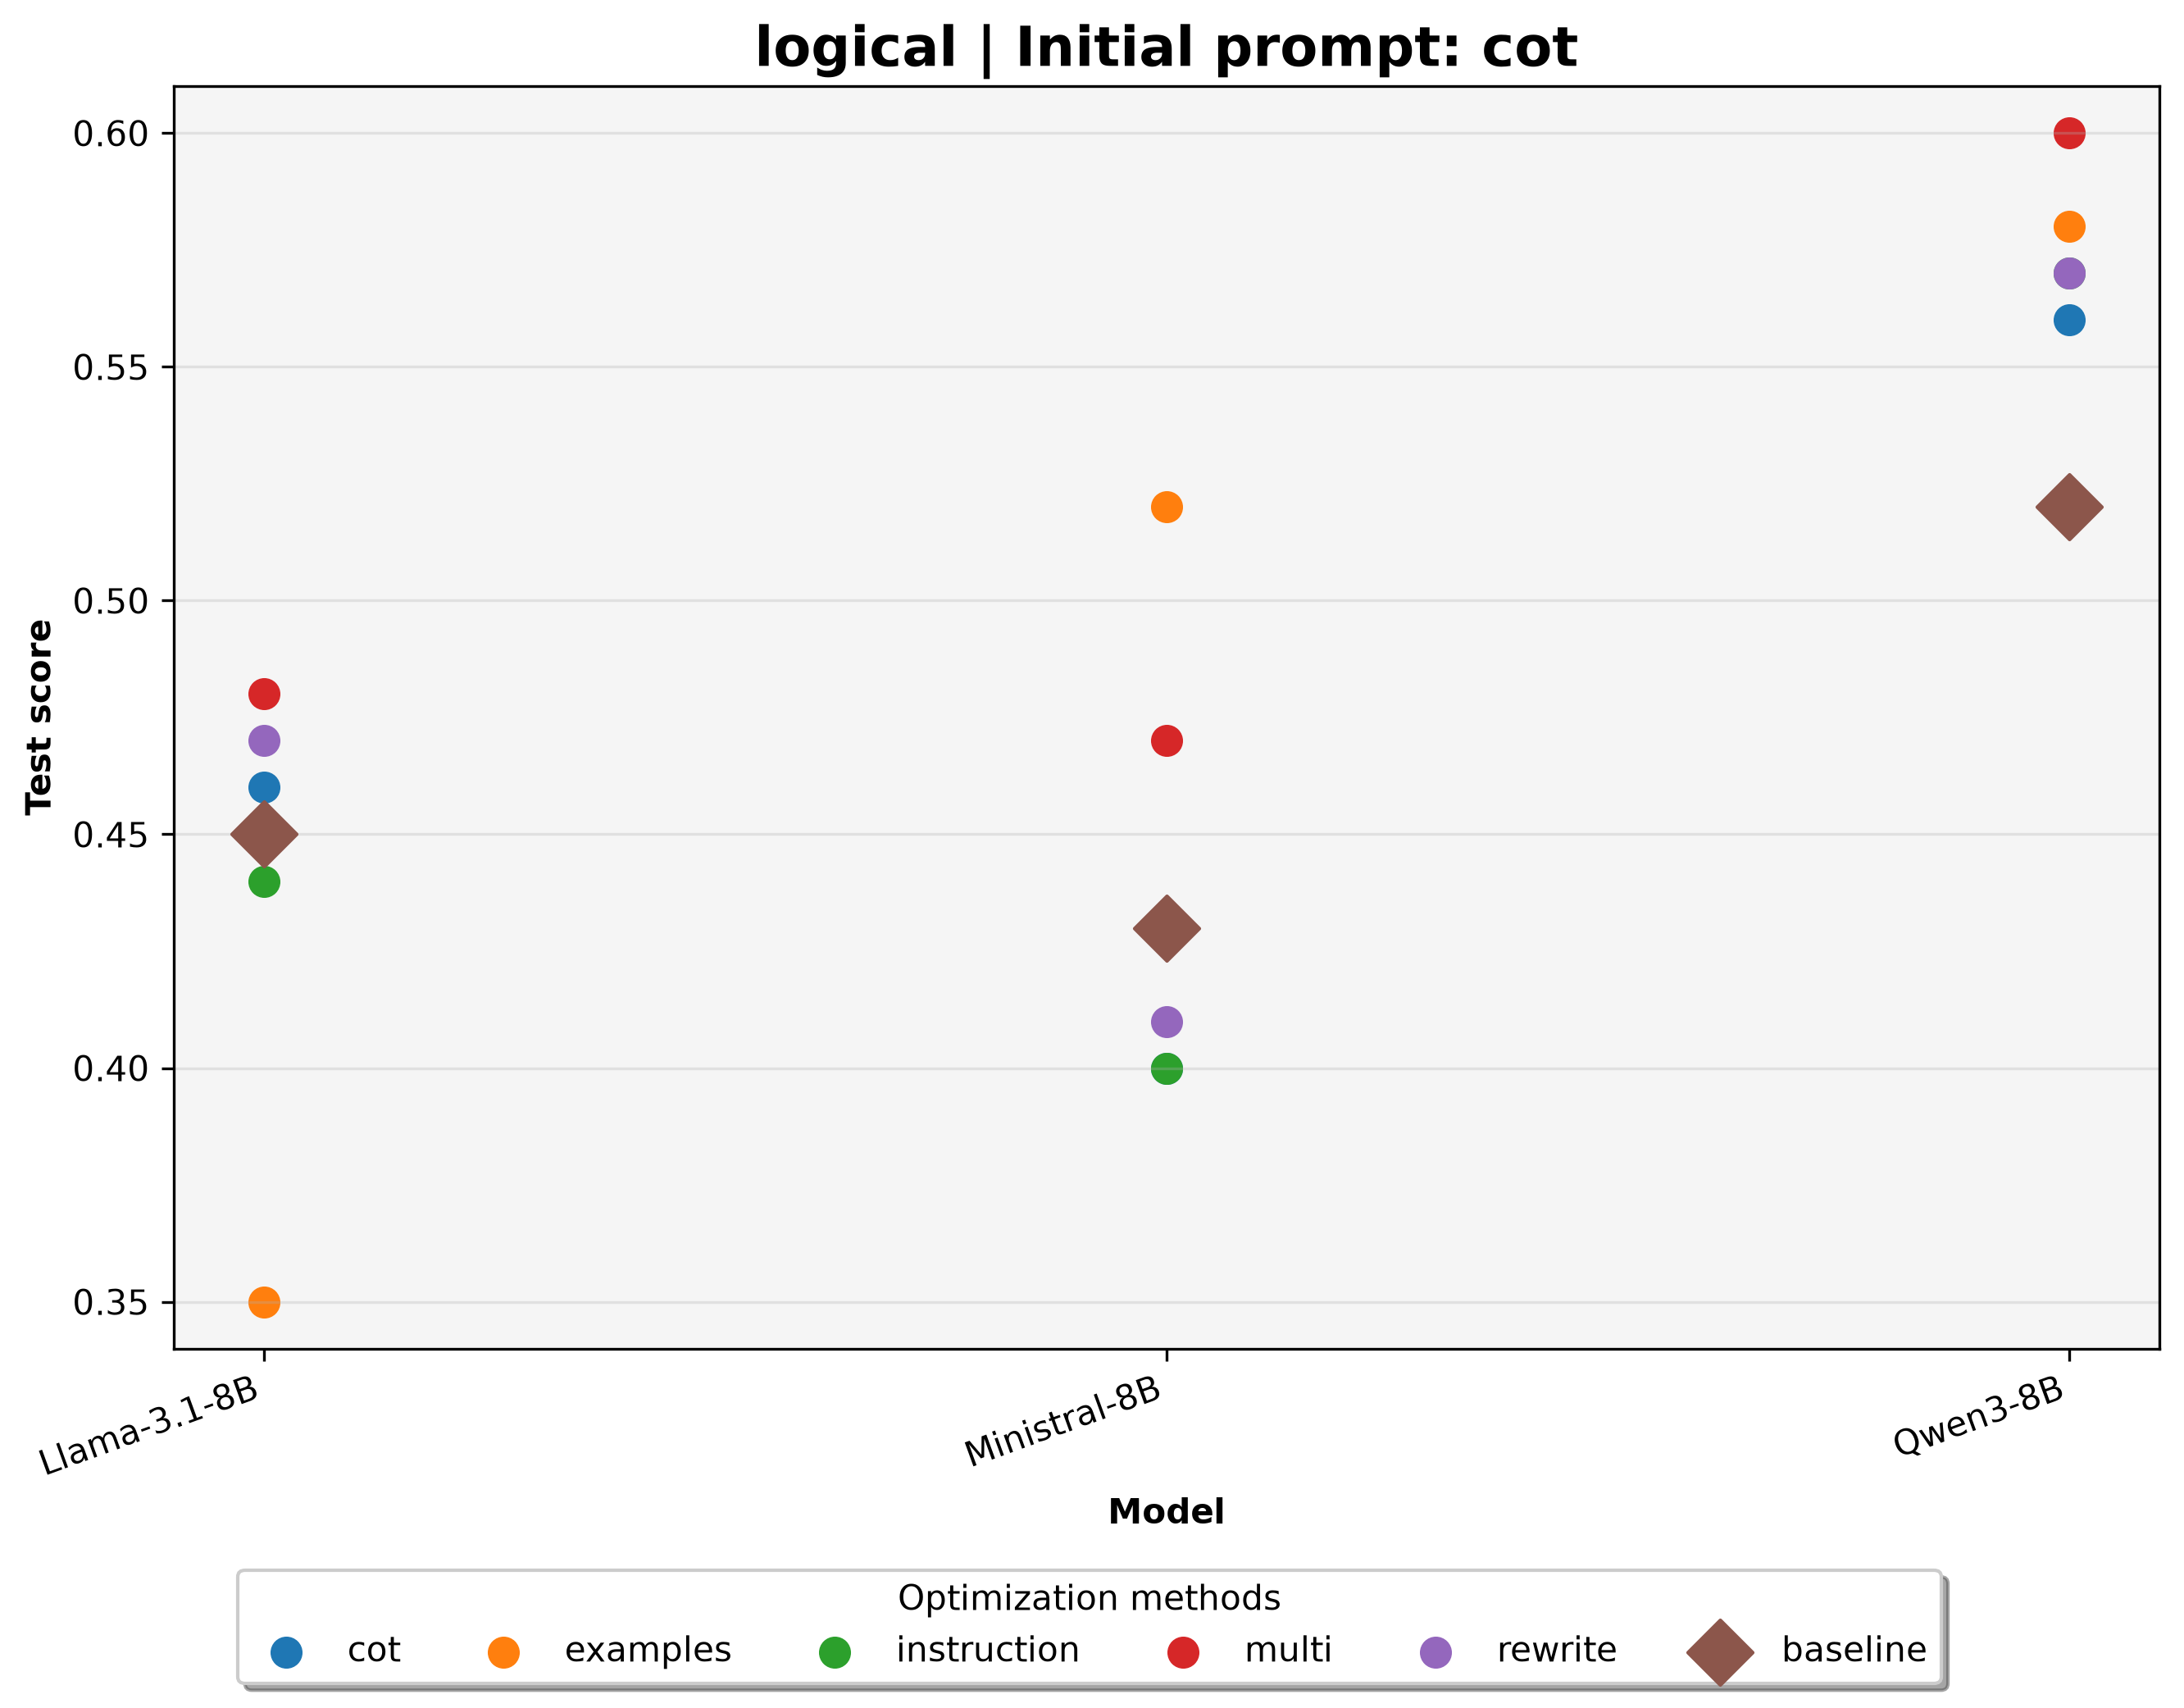
\includegraphics[width=0.90\textwidth]{../analysis/test_scores/logical_cot_test_scores.png}
%%}{}
%%\caption{Held-out test scores for the logical deduction task
%%starting from the CoT prompt.}
%%\label{fig:test_scores}
%%\end{figure}

For sentiment classification, several configurations generalize well.
For example, the Llama CoT prompt improves from $0.72$ to $0.79$ with the
multi-branch configuration, while the Ministral few-shot prompt improves
from $0.67$ to $0.77$ with the rewrite strategy. The Qwen few-shot prompt
also improves from $0.67$ to $0.75$ with the multi-branch configuration.
However, improvements are not guaranteed: the Llama zero-shot prompt
with the examples configuration decreases from $0.79$ to $0.77$.

The logical deduction task shows similarly strong variation. The Qwen
CoT prompt improves from $0.53$ to $0.60$ with the multi-branch
configuration, while the Ministral CoT prompt improves from $0.43$ to
$0.52$ with the examples configuration. Smaller improvements are also
observed in other configurations, such as the Qwen zero-shot prompt
with rewrite, which increases from $0.57$ to $0.58$. In contrast, some
optimized prompts perform worse on the held-out set. For example, the
Llama CoT prompt reaches only $0.35$ with the examples configuration,
despite the corresponding optimization improving its score on the
optimization set, while the Qwen zero-shot prompt decreases from $0.57$
to $0.52$ with the multi-branch configuration.

%%\begin{table}[htbp]
%%\centering
%%\caption{Representative held-out test results.}
%%\label{tab:test_results}
%%\begin{tabular}{llllrr}
%%\toprule
%%\textbf{Task} & \textbf{Model} & \textbf{Initial}
%%& \textbf{Configuration} & \textbf{Baseline} & \textbf{Final} \\
%%\midrule

    %%Sentiment
    %%& Llama
    %%& CoT
    %%& Multi
    %%& 0.72
    %%& 0.79 \\

    %%Sentiment
    %%& Ministral
    %%& Few-shot
    %%& Rewrite
    %%& 0.67
    %%& 0.77 \\

    %%Sentiment
    %%& Qwen
    %%& Few-shot
    %%& Multi
    %%& 0.67
    %%& 0.75 \\

    %%Sentiment
    %%& Llama
    %%& Zero-shot
    %%& Examples
    %%& 0.79
    %%& 0.77 \\

    %%Logical
    %%& Llama
    %%& CoT
    %%& Multi
    %%& 0.45
    %%& 0.48 \\

    %%Logical
    %%& Ministral
    %%& CoT
    %%& Examples
    %%& 0.43
    %%& 0.52 \\

    %%Logical
    %%& Qwen
    %%& CoT
    %%& Multi
    %%& 0.53
    %%& 0.60 \\

    %%Logical
    %%& Llama
    %%& Zero-shot
    %%& Examples
    %%& 0.47
    %%& 0.49 \\

    %%Logical
    %%& Ministral
    %%& Zero-shot
    %%& Instruction
    %%& 0.48
    %%& 0.41 \\

    %%Logical
    %%& Qwen
    %%& Zero-shot
    %%& Rewrite
    %%& 0.57
    %%& 0.58 \\

    %%\bottomrule
%%\end{tabular}

%%\end{table}

These results show that optimization on the 300-example search set is
not sufficient to guarantee generalization to unseen instances. They
also confirm that no single optimization strategy consistently
outperforms the others across all models and tasks. The effectiveness
of a mutation strategy depends strongly on the prompt from which the
search begins as well as on the characteristics of the task and model.

\paragraph{Mutation-Level Analysis}

The third part of the analysis considers the individual mutations rather 
than only the best prompt retained at each generation. The corresponding 
mutation-level plots are stored in the \texttt{analysis/improvement\_rate/} 
folder of the repository. A mutation is counted as an improvement if the 
child prompt scores higher than its reference score. For an ordinary
mutation, which has a single parent, the condition is:

$$
\text{child score} > \text{parent score}.
$$

For crossover, which has two parents, the comparison is made with the mean 
of the two parent scores:

$$
\text{child score}
>
\frac{\text{parent score}_1+\text{parent score}_2}{2}.
$$

The improvement rate of each optimization branch is the proportion of its 
mutations that satisfy this condition.

The total number of generated child prompts is not the same across models, 
initial prompts, or optimization branches, primarily because of the 
early-stopping mechanism. The instruction, CoT, and examples branches 
account for a larger number of mutations because they are evaluated both 
in their standalone configurations and together in the multi configuration, 
whereas crossover is available only in the multi configuration and 
generates relatively few children.

%%\begin{figure}[htbp]
%%\centering
%%\IfFileExists{../analysis/improvement_rate/sentiment_few_shots_improvement_rate.png}{
%%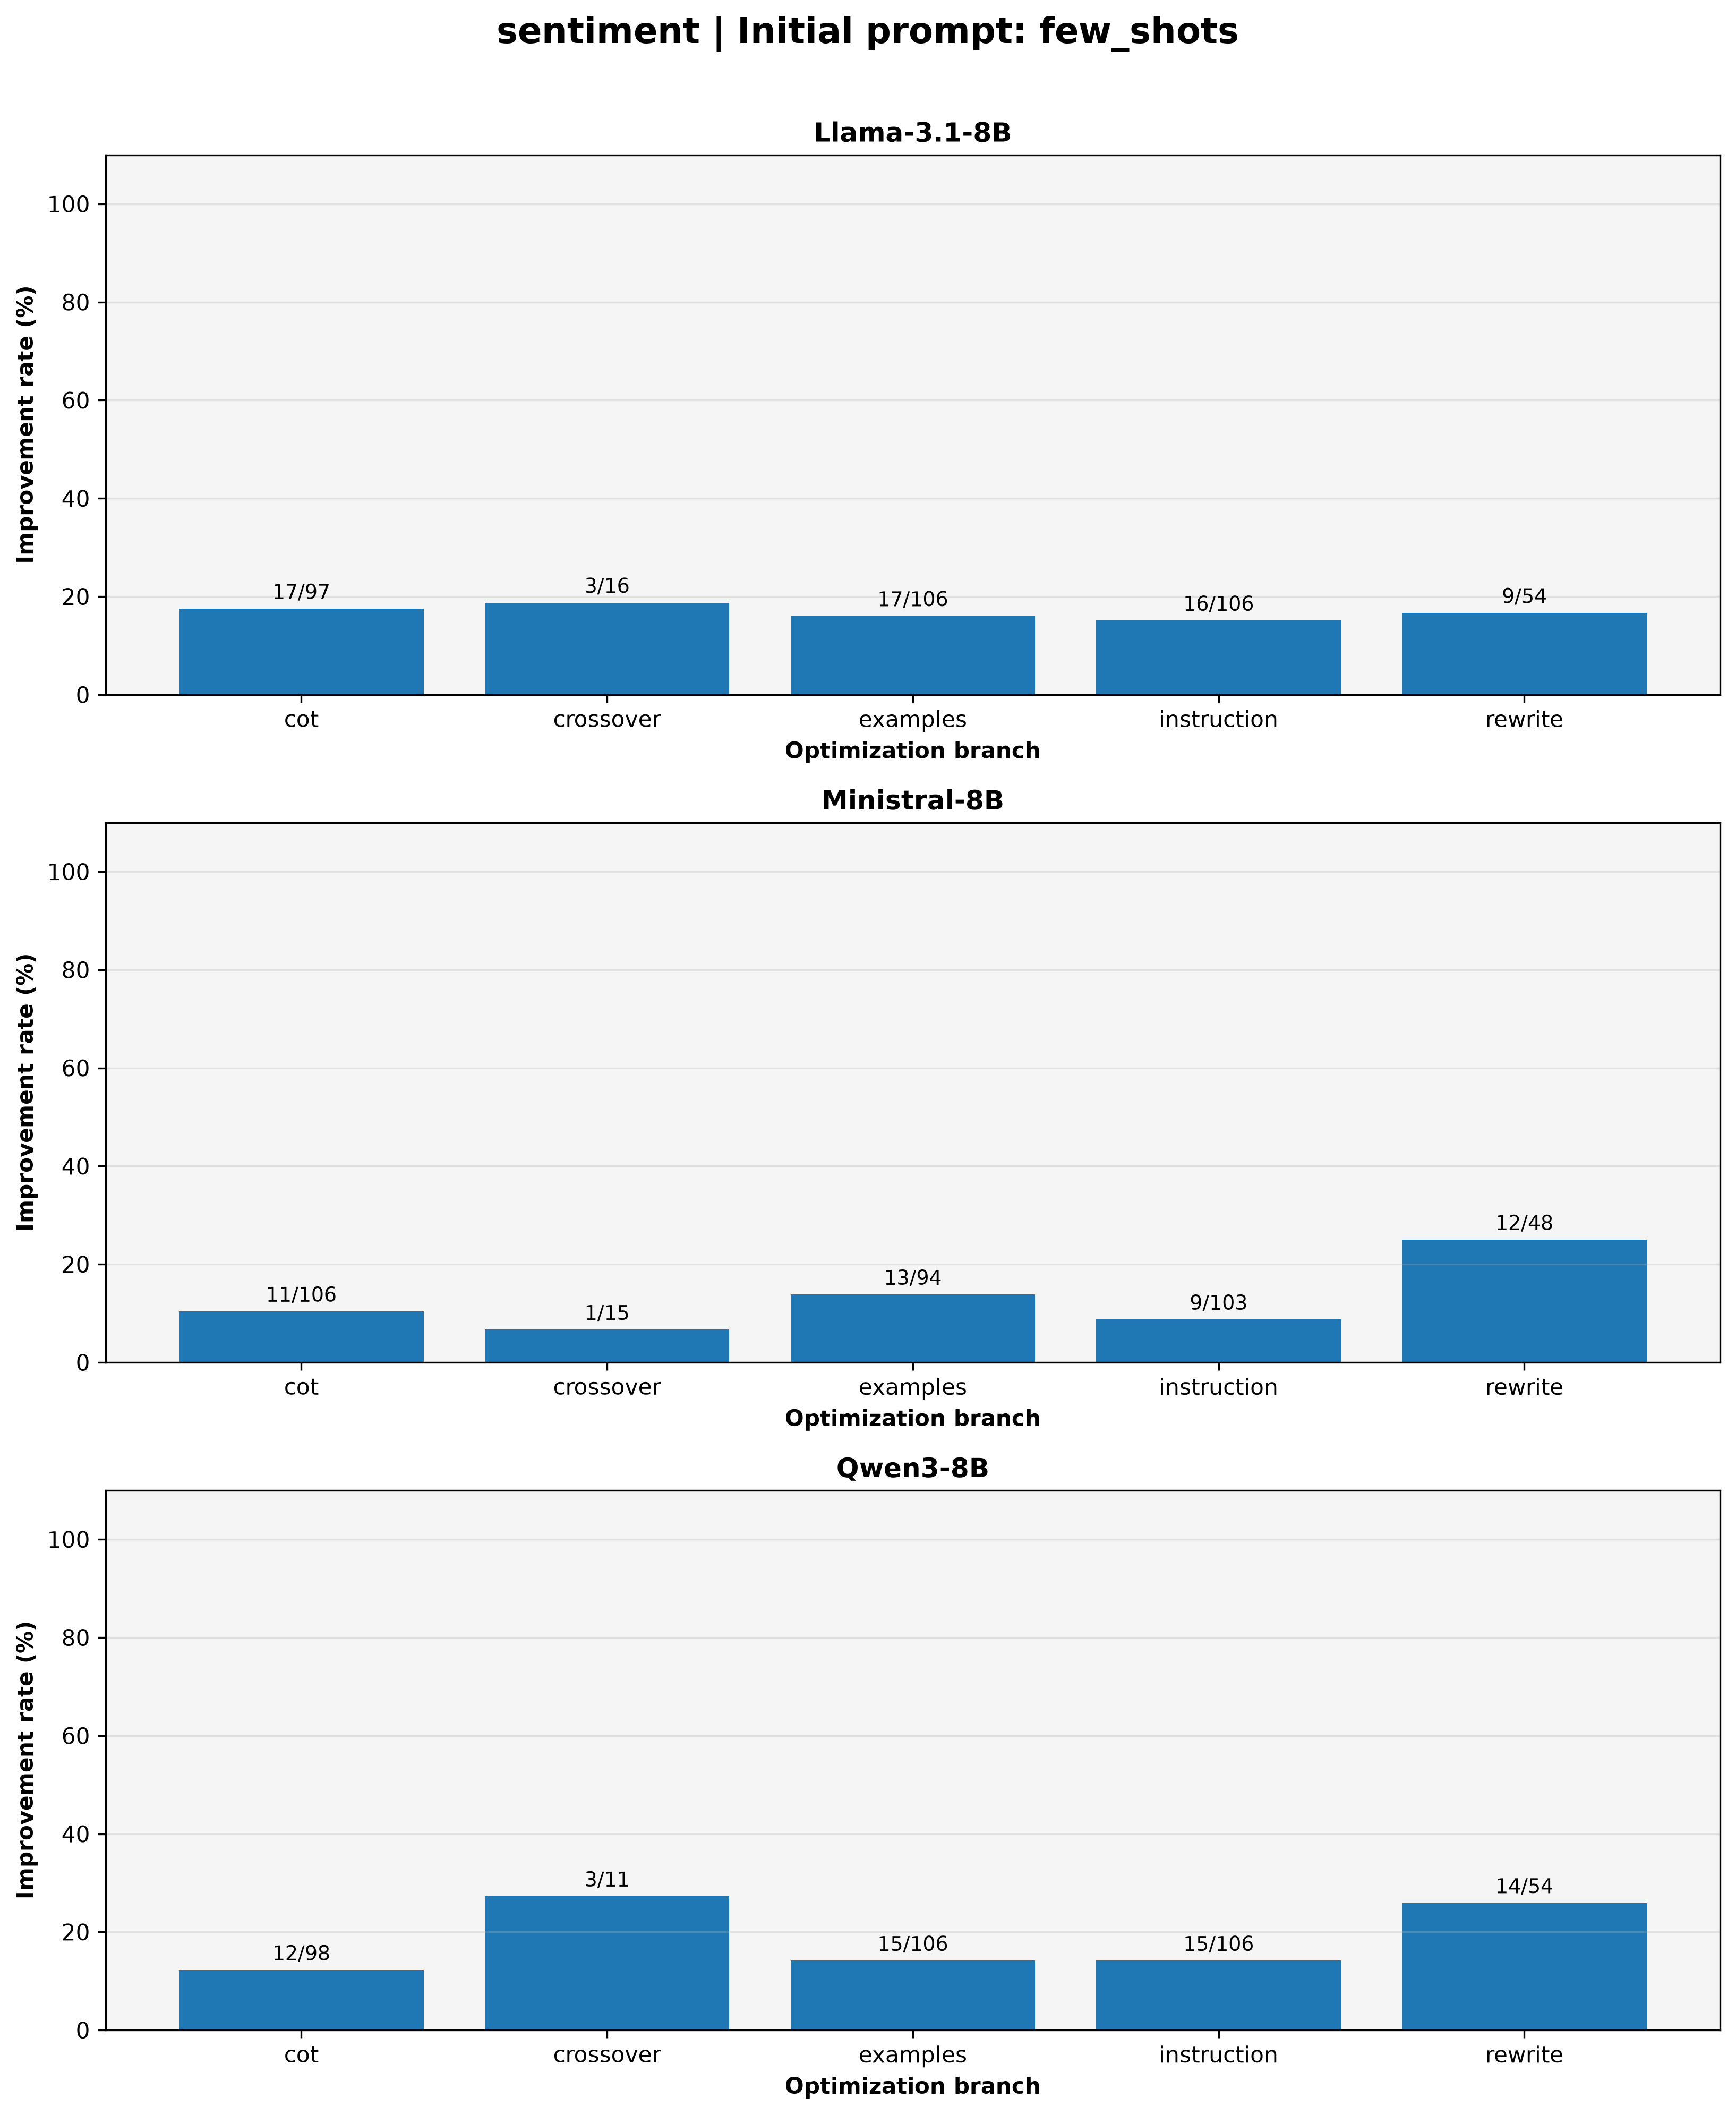
\includegraphics[width=0.90\textwidth]{../analysis/improvement_rate/sentiment_few_shots_improvement_rate.png}
%%}{}
%%\caption{Mutation improvement rates for the sentiment task
%%starting from the few-shot prompt.}
%%\label{fig:improvement_rate}
%%\end{figure}

This analysis complements the generation-level optimization curves.
The optimization-evolution plots show whether the best retained prompt
improves over time, while the mutation analysis shows how frequently
the individual branches generate a child that is better than its
reference parent.

A branch can therefore have a relatively low improvement rate while
still occasionally generating a high-scoring child that enters the
top-$k$ pool.

\section{Concluding remarks}

The experiments show that automated prompt optimization can modify the
performance of the evaluated models, but the effect is strongly
dependent on the task, model, initial prompt, and optimization method.

On the optimization dataset, improvements are generally modest. The
search process frequently produces prompts that are only marginally
better than the corresponding initial prompt, while a number of
configurations fail to find any prompt that exceeds the baseline.

The held-out evaluation shows why this optimization-set result cannot
be considered sufficient by itself. Some improvements transfer to
unseen examples, while others disappear or reverse.

The multi-branch strategy is frequently effective during optimization,
especially for the zero-shot and CoT configurations. However, the
held-out results do not show a universal advantage for this strategy.
Single-component optimization can also produce strong results in
specific conditions. The examples branch is particularly notable on
the logical task, while CoT and full prompt rewrite also provide strong 
results for selected models and initial prompts.

The initial prompt is therefore an important determinant of the
optimization outcome. The same optimizer can behave differently when
starting from zero-shot, CoT, or few-shot prompting. Similarly, the
same branch can be effective for one model and ineffective for
another.

The evaluation was limited to lightweight language models with
approximately 8 billion parameters. Consequently, the observed
behavior characterizes the proposed pipeline only within this model
scale. More capable and larger models may respond differently to prompt
mutations and could potentially provide larger or more consistent
improvements. The pipeline could also be further modified to better
exploit the capabilities and characteristics of more complex models.


\clearpage

\begin{thebibliography}{9}

      \bibitem{ye2024}
      Q. Ye, M. Ahmed, R. Pryzant, and F. Khani.
      \textit{Prompt Engineering a Prompt Engineer}.
      In \textit{Findings of the Association for Computational Linguistics: ACL 2024},
      pp. 355--385, 2024.
      \url{https://aclanthology.org/2024.findings-acl.21/}
      
      \bibitem{hsieh2024}
      C.-J. Hsieh, S. Si, F. Yu, and I. Dhillon.
      \textit{Automatic Engineering of Long Prompts}.
      In \textit{Findings of the Association for Computational Linguistics: ACL 2024},
      pp. 10672--10685, 2024.
      \url{https://aclanthology.org/2024.findings-acl.634/}
      
      \bibitem{schulhoff2024}
      S. Schulhoff, M. Ilie, N. Balepur, K. Kahadze, A. Liu, C. Si, et al.
      \textit{The Prompt Report: A Systematic Survey of Prompt Engineering Techniques}.
      arXiv preprint arXiv:2406.06608, 2024.
      \url{https://arxiv.org/abs/2406.06608}
      
      \bibitem{openai-chatgpt}
      OpenAI.
      \textit{ChatGPT}.
      \url{https://chatgpt.com/}
      
      \bibitem{hf-qwen}
      Hugging Face.
      \textit{Qwen/Qwen3-8B-GGUF}.
      \url{https://huggingface.co/Qwen/Qwen3-8B-GGUF}
      
      \bibitem{hf-llama}
      Hugging Face.
      \textit{m2wws/Llama-3.1-8B-Instruct-Q4\_K\_M-GGUF}.
      \url{https://huggingface.co/m2wws/Llama-3.1-8B-Instruct-Q4_K_M-GGUF}
      
      \bibitem{hf-ministral}
      Hugging Face.
      \textit{DuoNeural/Ministral-8B-Instruct-GGUF}.
      \url{https://huggingface.co/DuoNeural/Ministral-8B-Instruct-GGUF}
      
\end{thebibliography}

\end{document}
